
\section{Misc}

\subsection{Going further on defining conflict}
We defined earlier that we would consider only edge and node conflict. Thus we can redefine them and add some variant; being able to have more information about a conflict might help us solving them or makes the selection of heuristics more robust (see~\ref{subsec:selecting_heuristic}). The first type of conflict hat we can identify is a conflict that can be solved using only wait move\footnote{It is of course not the only way, or even always the most efficient way of solving this kind of conflict} (see~\ref{img:waitconflict}). Formally, a  node ``wait-conflict'' \(c_{wait}\) occurs between agent \(a\) and \(a'\), if at time step \(t\),  \(\pi_a[t] = \pi_{a'}[t]\) and if \(\pi_a[t+1] != \pi_{a'}[t-1]\) and \(\pi_a[t-1] != \pi_{a'}[t+1]\). By definition, edge conflict can not be solved using wait only move. We can then consider the ``dodge conflict'', in contrary to the ``wait conflict'', ``dodge conflict'' can only be solved by extending the plan with unvisited node of the graph (in other words, extending the subgraph defined by a given path). Formally, node ``dodge conflict'' \(c_{dodge}\) occurs between agent \(a\) and \(a'\), if at time step \(t\),  \(\pi_a[t] = \pi_{a'}[t]\) and if \(\pi_a[t+1] = \pi_{a'}[t-1]\) and \(\pi_a[t-1] != \pi_{a'}[t+1]\). Edge conflict are by defnition ``dodge conflict''.

We can also identify reccuring conflict

Statment
\begin{itemize}
  \item Considering two paths of distinct agent, if they have more than 1 dodge conflicts, these paths are not shortest path. (I think)
  \item If two agents have dodge conflict, swapping their goals is an interesting move
  \item 
\end{itemize}






\begin{figure}[H]
  \centering
  \caption{Example of wait conflict and an example solution}\label{img:waitconflict}
  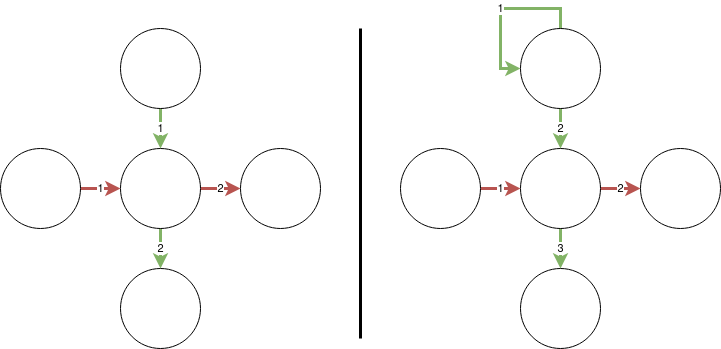
\includegraphics[width=\widthimg]{img/WaitConflict.drawio.png}
\end{figure}






\subsection{Selecting heuristic considering the MAPF problem}\label{subsec:selecting_heuristic}
Considering two MAPF problems \(A\) and \(B\), it is evident that a heuristic might be very effective for solving \(A\) but have no interest being used in \(B\). This can be due the graph (high/low density of obstacles, the size, etc), the number of agents, their disposition\ldots Hoever we can try to order or select the heuristics/approaches. Considering the reason enumerated above we can draw different metrics than might help selecting the heuristics/approaches:
\begin{itemize}
  \item Density of obstacles: can be computated by counting the average degree for each node of the graph.
  \item The size of the graph: can be computed by counting the number of nodes
  \item The disposition of the agents:\begin{itemize}
    \item We can count the number of groups that we can create (based on meta-agent technique or simple distance average selection)
    \item Average distance between agent (might need to be combined with a grouping techinque if agents a disposed at the edges of the graph)
  \end{itemize}
  \item Considering the kind of conflict
  \item others?
 \end{itemize} 

From the approaches that we defined, we can tell that corridor extention would not be selected if the density of obstacle is high (see~\ref{img:blocking_agent}).





\subsection{Others}
\subsubsection{Time expanded graphs}
Need to explore more about this; how it can help solving the problem, what are the kind of path that would be interesting as input, what merging strategies can be applied..

\subsubsection{Highway}
\begin{itemize}
  \item Summary: Highway\cite{coko16a,courkuxuayko16a} heuristic aims to change the graph by remove edges resulting with part of the graph that become oriented.
  \item Require: using following conflict paths might create better highway especially on self generated\cite{courkuxuayko16a} ones.
  \begin{figure}[H]
    \centering
    \caption{Example of highway (figure 2 of paper\cite{coko16a})}\label{img:highway}
    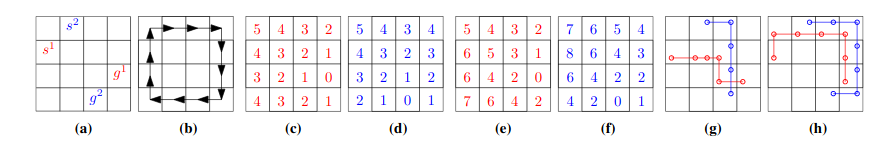
\includegraphics[width=\widthimg]{img/highways.png}
  \end{figure}
\end{itemize}


\subsubsection{Pruning by pulling goal}
\begin{itemize}
  \item Summary: Considering a agent and its path, each step both the goal and the agent are moving toward each other until a path or plan conflict occurs. Once a conflict is found, we use the position of the goal and the position of the agent to a rectangle (being the diagonal).
  \item Require: feels like it could only work for one path at the time, otherwise it might take too much computation time. 
  \begin{figure}[H]
    \centering
    \caption{Example of goal pulling}\label{img:pulling_goal}
    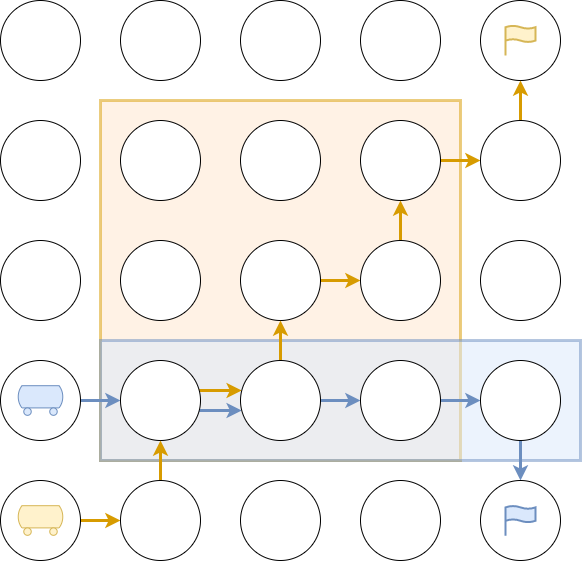
\includegraphics[width=\widthimg]{img/puling_goal.drawio.png}
  \end{figure}
\end{itemize}

\subsubsection{Loop Highway 14-Loyd-Puzzle, Carousel}
\begin{itemize}
  \item Idea: considering a path that goes through every starting position and goal position of every agents, loop, and do not cross; we can maybe assume that if the loop has two distinct conflict-free vertices neighboring the loop, their is a solution. If we consider that agent disappear on goal, it is an even better solution. If we can create the loop talked about above we are in a situation in worst case of the 14-Loyd-puzzle that I assume is solvable whatever the configuration. We can also consider multiple loops.
\end{itemize}

\begin{figure}[H]
  \centering
  \caption{Example of one loop and two loops}\label{img:loyd_loop}
  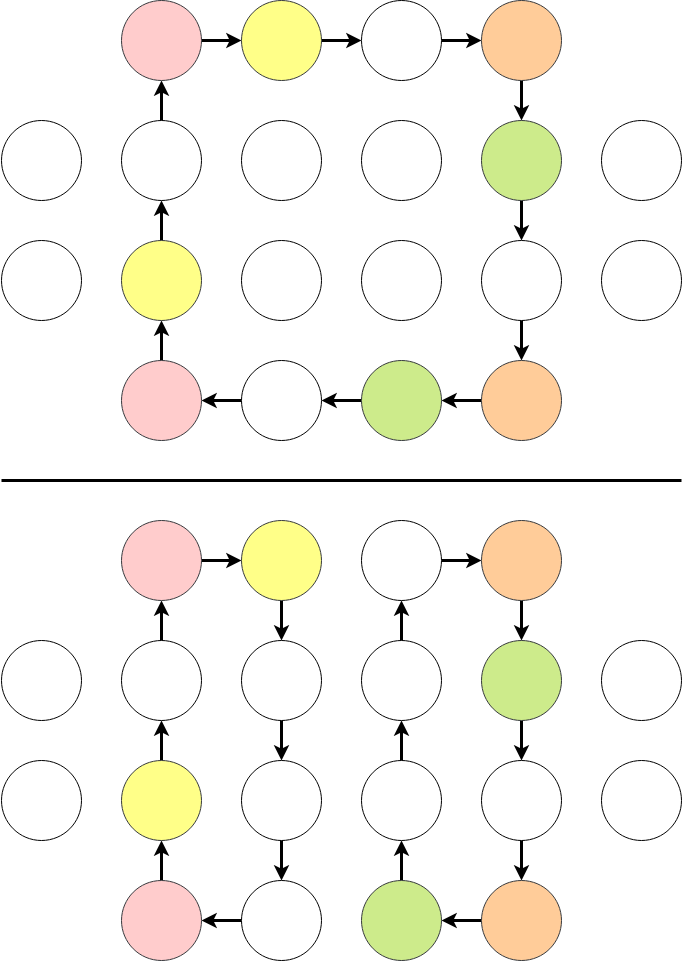
\includegraphics[width=\widthimg]{img/loop_highway.drawio.png}
\end{figure}

                             
\subsubsection{Waiting only}
\begin{itemize}
  \item Summary: the agents are only allowed to wait, no sub-graph extension is allowed.
  \item Require: In order to raise the chances of finding a solution, we need a higher number of diverse path, however, som problems can't  be solved through waiting, and some problem could be solved by waiting a huge amount of time. 
  \item Variant:\begin{itemize}
    \item Fixing waiting position with time interval\cite{phli11a,naphli12a}
    
    
    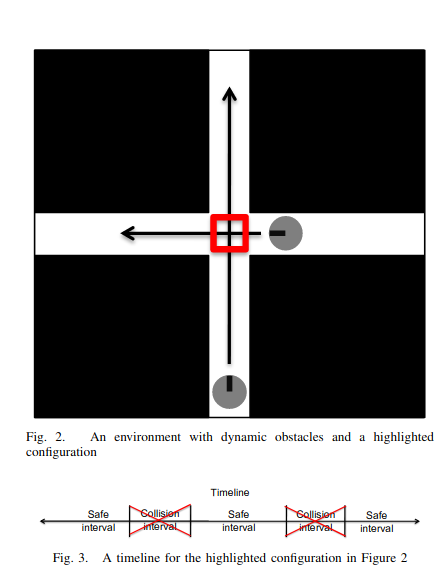
\includegraphics[width=5cm]{img/safeinterval.png}
    \item Fixing waiting position based on conflict free zone
  \end{itemize} 
\end{itemize}



\subsection{Guiding the agents}
\subsubsection{Heatmap}

\begin{itemize}
  \item Summary: The idea is to create for each vertices of the graph, an indicator that would describe how much the vertex ``used'' b y the agents. We can imagine something like, for each vertex, we have the number of time step where an agent is at the vertex divided by the makespan. The idea would then be to \begin{itemize}
    \item guide the agents using the indicator (the indicator may refer to the probability of presence of another agent)
    \item guide the graph extension by choosing the vertices that have a lower or higher ``usage''
  \end{itemize}
  \item Require: at least one path for each agents, the more paths we have the more precise the heatmap can be.
  \item Variants: \begin{itemize}
    \item Take into consideration the robustness~\cite{atstfewabazh20a,atstfestko20a}
    \item make the heatmap evolve over time step
  \end{itemize} 
\end{itemize}



\subsubsection{From the bachelor thesis}
\begin{itemize}
  \item Deathlaser: the idea is to keep the agents at a closer position from their goal by pruning their subgraph around their previous position, probably require only 1 paths
  \item Homesick: the idea is to force the agent to come back to their plan after $t$ time not being on their original plan. Might require a graph extension beforehand 
  \item Checkpoints (or Divide and Conquer~\cite{yulav16a}): the idea is to add $n$ ``checkpoint'' vertices on the original path where their final paths should contains these vertices. Work only with one path 
\end{itemize}


